\section{Diagnostic set C: calibration eligibility and label reuse}
Ten additional replays cross the frozen and original head scores with ALL256 and ALL256-G. The head trajectory, requests and delay remain fixed. ALL256 uses its own minimum-per-class gate; ALL256-G uses the head gate. Both accept every acquired label, whereas ROLE256 accepts only CAL-role arrivals. A parallel audit buffer verifies identical ALL256 retention and measures overlap with the current FIT192 feature digests; it does not supply data to the controller. The shared trajectories match diagnostic set B exactly. Per-block counts, thresholds, head-state digests, normal-role errors, and the overlap ledger are retained in diagnostic set C.

\begin{table}[tb]
\centering\small\setlength{\tabcolsep}{4pt}
\caption{Normal-vector role allocation on D. Unique CAL and traffic CAL are percentages of unique normal vectors and normal occurrences respectively. The ten most frequent normal vectors account for 46.23\% of TON normal traffic and 18.03\% of UNSW normal traffic, independently of salt.}
\begin{tabular}{llrrr}\toprule
Stream & Salt & Unique vectors & Unique CAL (\%) & Traffic CAL (\%)\\\midrule
TON & Default & 87,132 & 25.19 & 31.05\\
TON & Salt 1 & 87,132 & 24.93 & 35.22\\
TON & Salt 2 & 87,132 & 24.99 & 17.59\\
UNSW & Default & 490,087 & 25.09 & 22.96\\
UNSW & Salt 1 & 490,087 & 25.12 & 23.18\\
UNSW & Salt 2 & 490,087 & 24.98 & 20.68\\
\bottomrule\end{tabular}
\end{table}

For TON at the 5\% target, the default role split has 213,509 FIT-role and 96,164 CAL-role normal observations. Frozen/ROLE256 yields mean FP counts of 91,534.8 and 7,496.4 respectively; Head/ROLE256 yields 25,187.0 and 9,538.4. Frozen/ALL256 yields 11,200.2 and 2,959.0, and Head/ALL256 yields 22,097.8 and 9,549.8. These are descriptive strata of the same evaluation observations. Roles are fixed by the input vector, so the counts are constant across label-query seeds at a fixed salt.

\begin{table}[tb]
\centering\small\setlength{\tabcolsep}{3pt}
\caption{All-label FPR-target controls, including the matched head gate (-G). Target and rates are percentages, mean $\pm$ conditional seed SD. Both score functions use the same calibration occurrences and update schedule within each pair.}
\begin{tabular}{llrrrr}\toprule
Stream & Controller & Target & Recall & FPR & BA\\\midrule
\tablerows{tables/all_label_target_rows.tex}
\bottomrule\end{tabular}
\end{table}

At $\lambda=1$ and 2, the ALL256-G score contrasts equal their independently gated ALL256 counterparts. This agreement is specific to the recorded trajectories; the gates are not defined to be identical. TON's independently gated thresholds improve BA by about 0.42 and 0.33 points respectively for both scores, compared with the head-gated versions. In the UNSW FPR-target traces there is a small gate difference at the 20\% target, while the two displayed cost weights coincide.

Within-seed all-label interpolation is restricted to common observed support. TON supports four pairs at 10\% FPR and five at 13\% and 20\%. UNSW supports none of these all-label targets on the recorded cost grid, so corresponding estimates remain missing. This is distinct from the direct causal target controllers in the preceding table. All-label calibration is evaluated under a permissive label-reuse contract: a head may use the same acquired labels in fitting and threshold selection. The future evaluation labels remain delayed and unavailable at prediction time.

\FloatBarrier
\subsection{Complete policy-package and prevalence summaries}
\begin{table}[tb]
\centering\small\setlength{\tabcolsep}{4pt}
\caption{Spline operating policies. Rates are percentages, mean $\pm$ sample SD across five randomizations conditional on each stream. Each threshold uses only past labels.}
\label{tab:costs}
\begin{tabular}{llrrr}\toprule
Stream & Policy & Recall & FPR & BA \\\midrule
\tablerows{tables/diagnostic_a_cost_rows.tex}
\bottomrule\end{tabular}
\end{table}

\begin{table}[tb]
\centering\small\setlength{\tabcolsep}{4pt}
\caption{Requested calibration FPR versus achieved future rates for the spline score. Target and rates are percentages. Mean $\pm$ sample SD describes five randomizations of the same stream. Thresholds use only previously available normal labels.}
\label{tab:fprtargets}
\begin{tabular}{lr l rrr}\toprule
Stream & Target & Controller & Recall & FPR & BA \\\midrule
\tablerows{tables/diagnostic_a_fpr_rows.tex}
\bottomrule\end{tabular}
\end{table}
Figure~\ref{fig:pr} reports precision--recall at the actual causal operating points. TON's attack-dominated prevalence can yield high precision despite a large FPR. To make that dependence visible, the third panel uses the same class-conditional rates at hypothetical 1\% prevalence:
\begin{equation}
 \mathrm{precision}(\pi)=\frac{\pi\,\mathrm{recall}}{\pi\,\mathrm{recall}+(1-\pi)\,\mathrm{FPR}}.
\end{equation}
For example, the TON head at $\lambda=1$ yields 4.37\% precision at 1\% prevalence and 0.45\% at 0.1\%. These are conditional calculations, not predictions for a new network.

\begin{figure}[tb]
\centering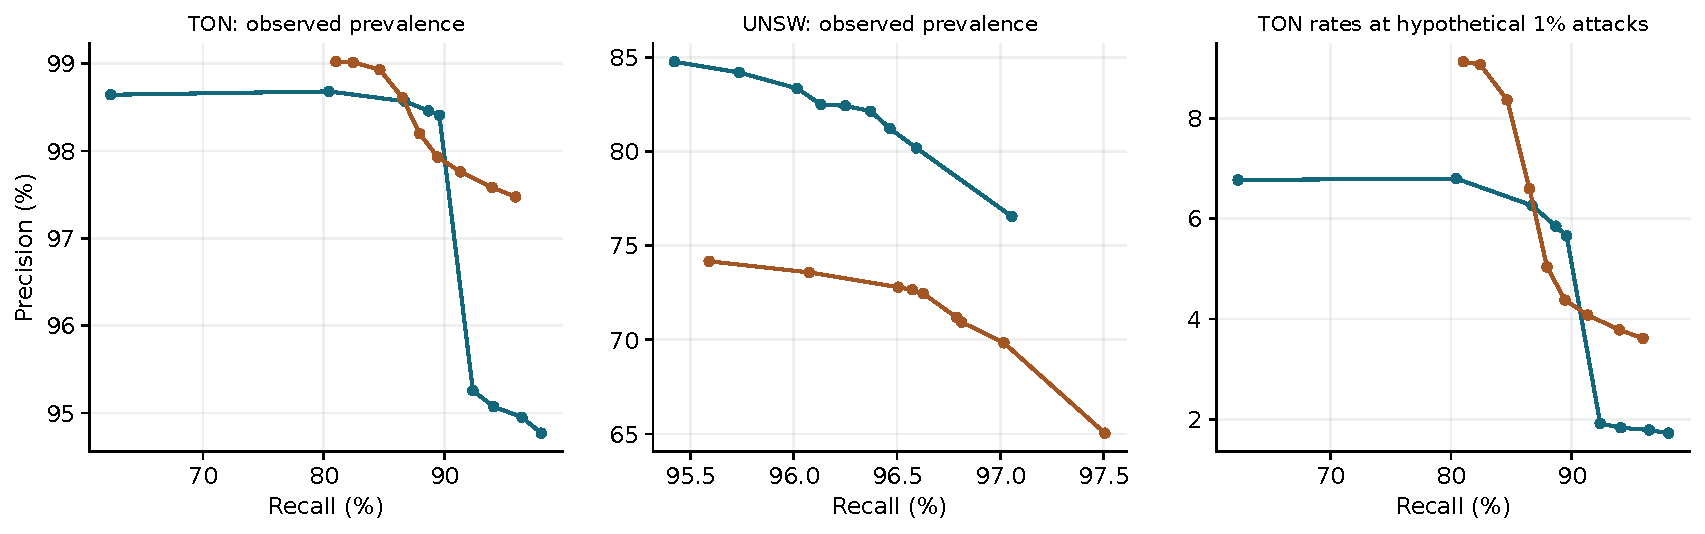
\includegraphics[width=\linewidth]{figures/diagnostic_a_precision_recall.pdf}
\caption{Precision--recall operating points selected by the fixed cost grid. The first two panels use observed class counts. The last panel assumes that TON's class-conditional rates transfer to 1\% attack prevalence. Points are seed means conditional on each capture; they are not pooled adaptive-score PR curves.}
\label{fig:pr}
\Description{Precision--recall operating points selected by the fixed cost grid. The first two panels use observed class counts. The last panel assumes that TON's class-conditional rates transfer to 1\% attack prevalence. Points are seed means conditional on each capture; they are not pooled adaptive-score PR curves.}
\end{figure}


